\section{System Architecture and Incentive Structure}
    The previous sections have described how Tagion solves the \gls{trilemma} by utilizing its unique features. While the previous sections have delved into specific parts of the system, the following section gives a broader overview of the system as a whole.

\subsection{Tagion from a User Perspective}
    If a user wants to use the Tagion system, the message must be communicated to one of the many nodes of the Tagion system. It is possible to build a relay system on top of the network, to make sure user messages are evenly distributed. A message can be anything from a transaction to a smart contract (a piece of executable code)\footnote{All things in the network are technically smart contracts. A transaction is just a piece of code telling the system to move tokens from A to B.}. The user must prove that its message is valid; that he owns the money he is using, or owns the file he is deleting. To do this the user submits a signature together with the message.

    \begin{figure}[H]
        \centering
        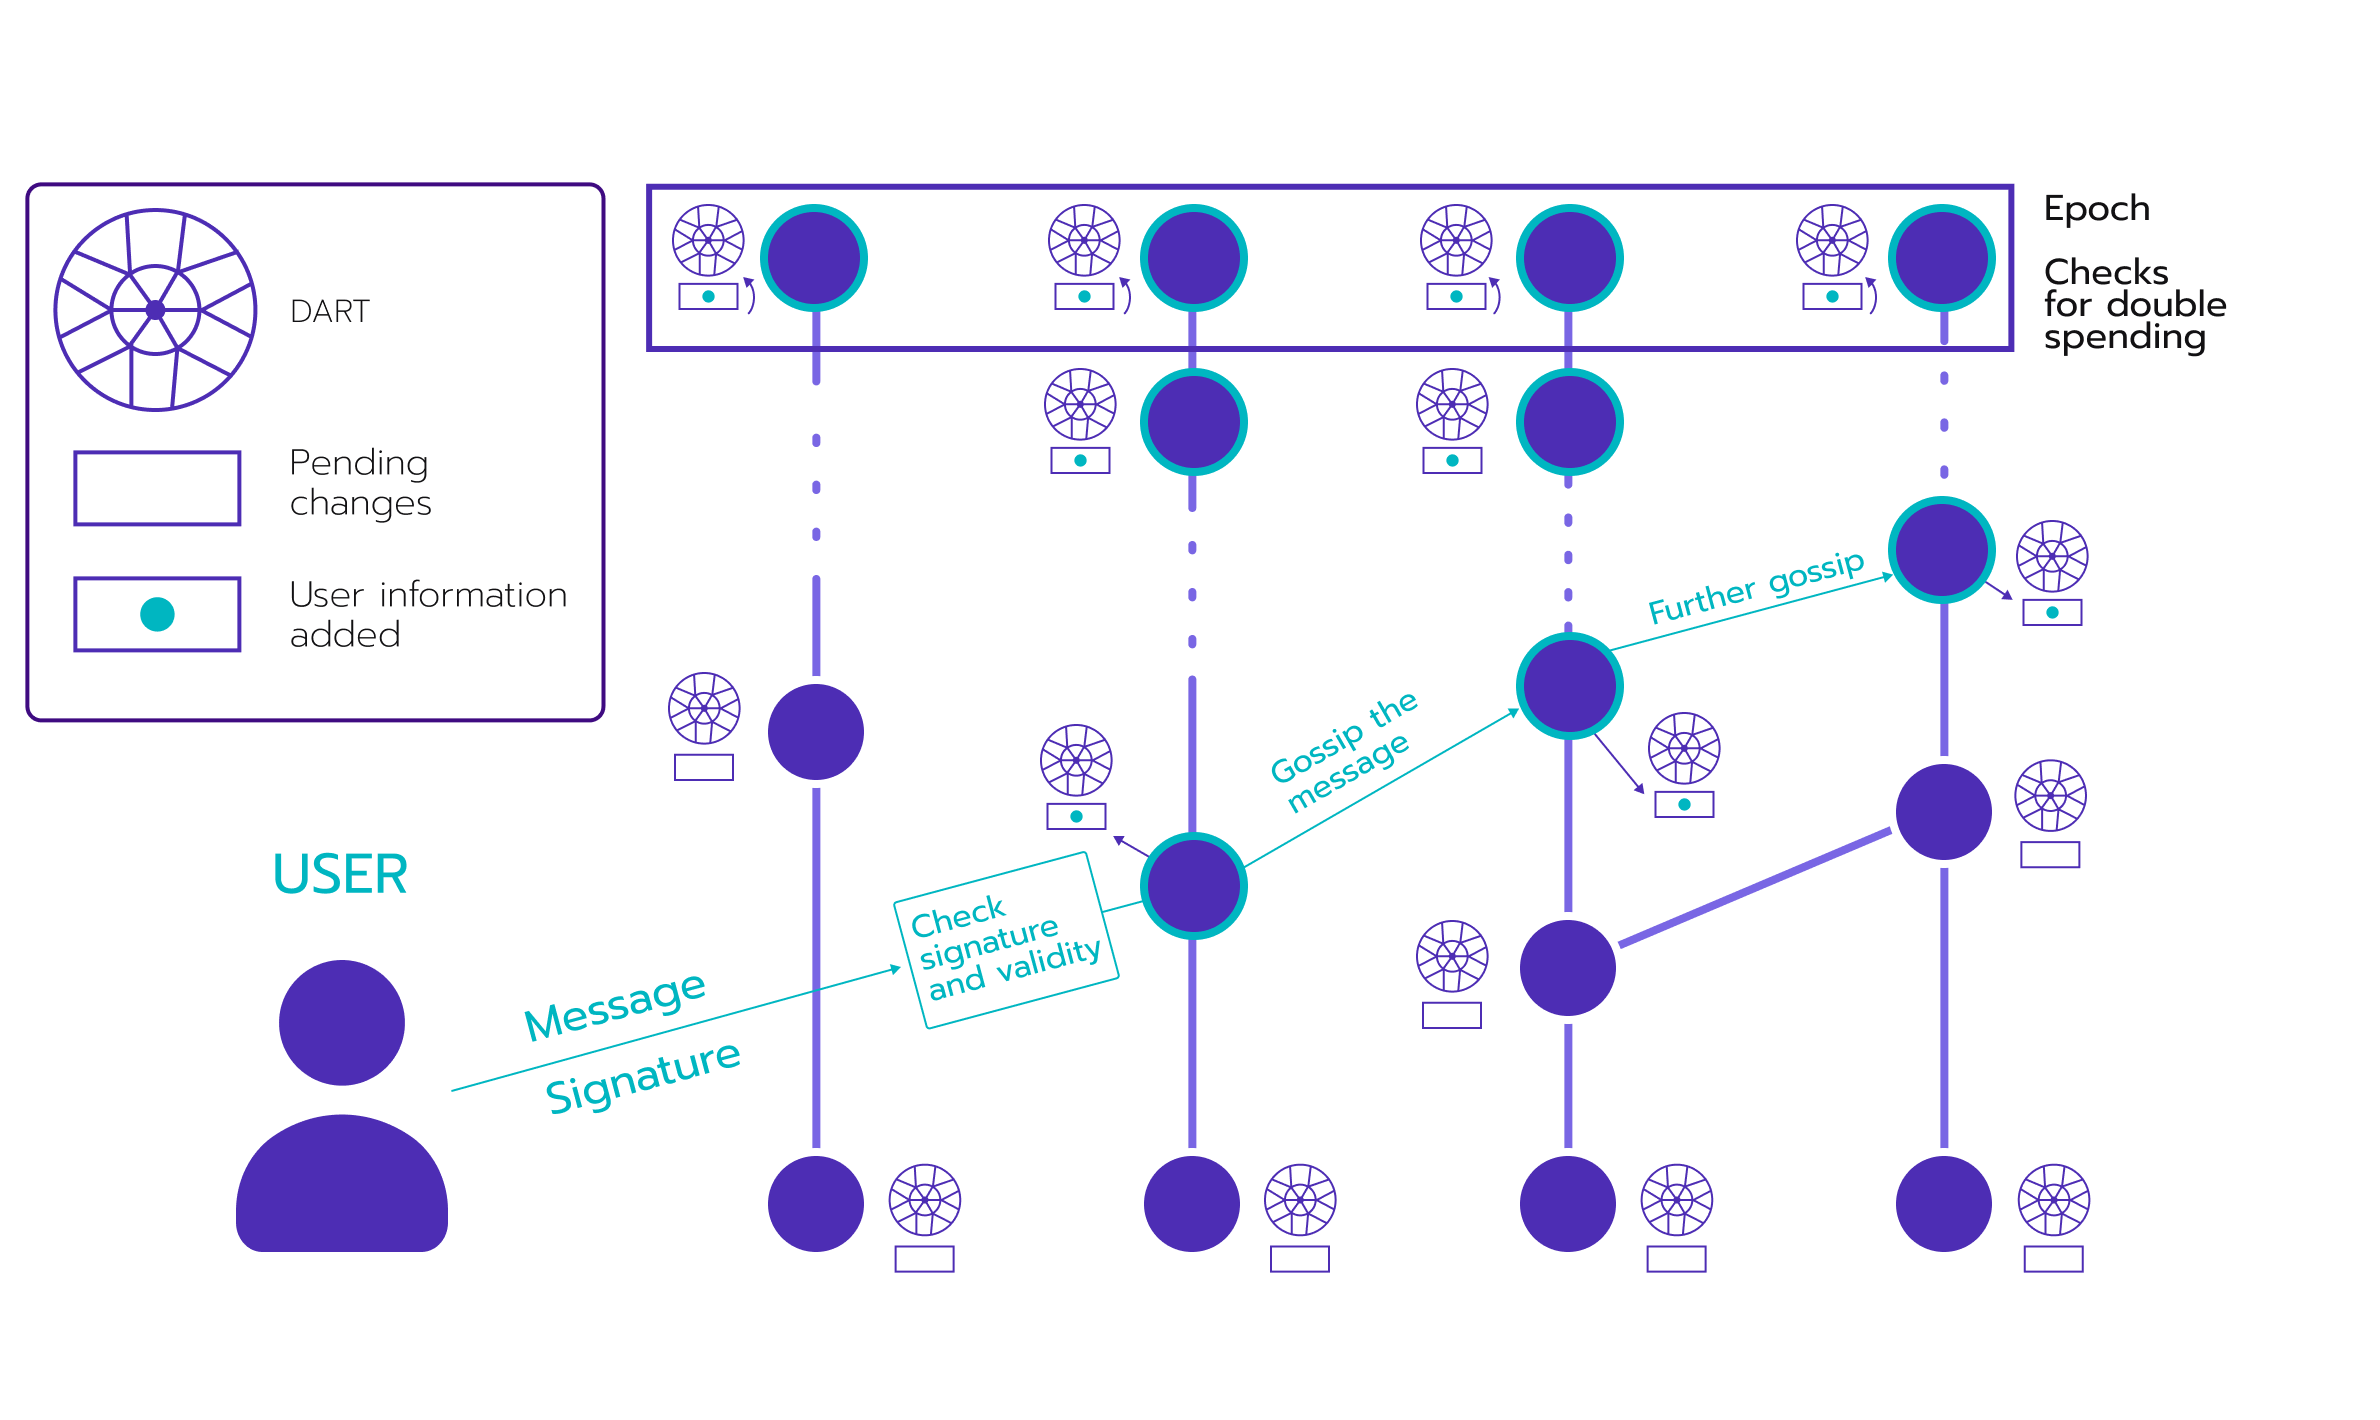
\includegraphics[width=1.2\textwidth,center]{figures/system_architecture.png}
        \caption{How a message flows from the user, until there is consensus about it in the network.}
        \label{figure:system_architecture}
    \end{figure}

    When a node receives a message it checks that the message is valid, and that the signature gives the correct permissions. If the node forwards an invalid message it will be penalized by the rest of the system, so it is incentivised to check the validity of the users message. When this check has been done, the node saves the user message in pending changes. As the network runs, gossip about the message spreads throughout the network. Whenever the message reaches a new node it does the same validity checks, and adds the message to its local pending changes.
    After some time, the message has spread to all nodes. When an epoch happens where every famous witness (actively participating) node has heard of the event, the event is permanently ordered with respect to other events. This allows the system to make a final check for double spending (that you have not spent the same bill twice) before it permanently writes the message from the pending changes into the \gls{dart}. At this point the message has achieved finality: The message is registered, ordered, and is mathematically certain to never be overridden. The following two sections zooms in on what happens on a low level from a node perspective. Firstly, when nodes receive messages, and secondly, when epochs occur.

\subsection{Node POV: Receiving Information}
    Nodes can receive information in two ways: Either from gossip inside the Hashgraph, or from user input. Gossip is transferred through the Wavefront Protocol described in section \hyperref[sec:scalability]{\underline{3. Scalability}}, and user input is just sent directly to the node. Either way, the received data is handled the same. The node passes the information through the execution pipeline. This module reads the input of the different smart contracts from the \gls{dart}. It uses this to check the validity of the provided signature, and the passed message is valid in general. Once the messages has passed all the tests, they are executed in the \gls{tvm}. This virtual machine executes the smart contracts and adds the output of these to the pending changes. Note how the storage layer of the system is separated into a structure (the \gls{dart}) outside the consensus layer.

    \begin{figure}[H]
        \centering
        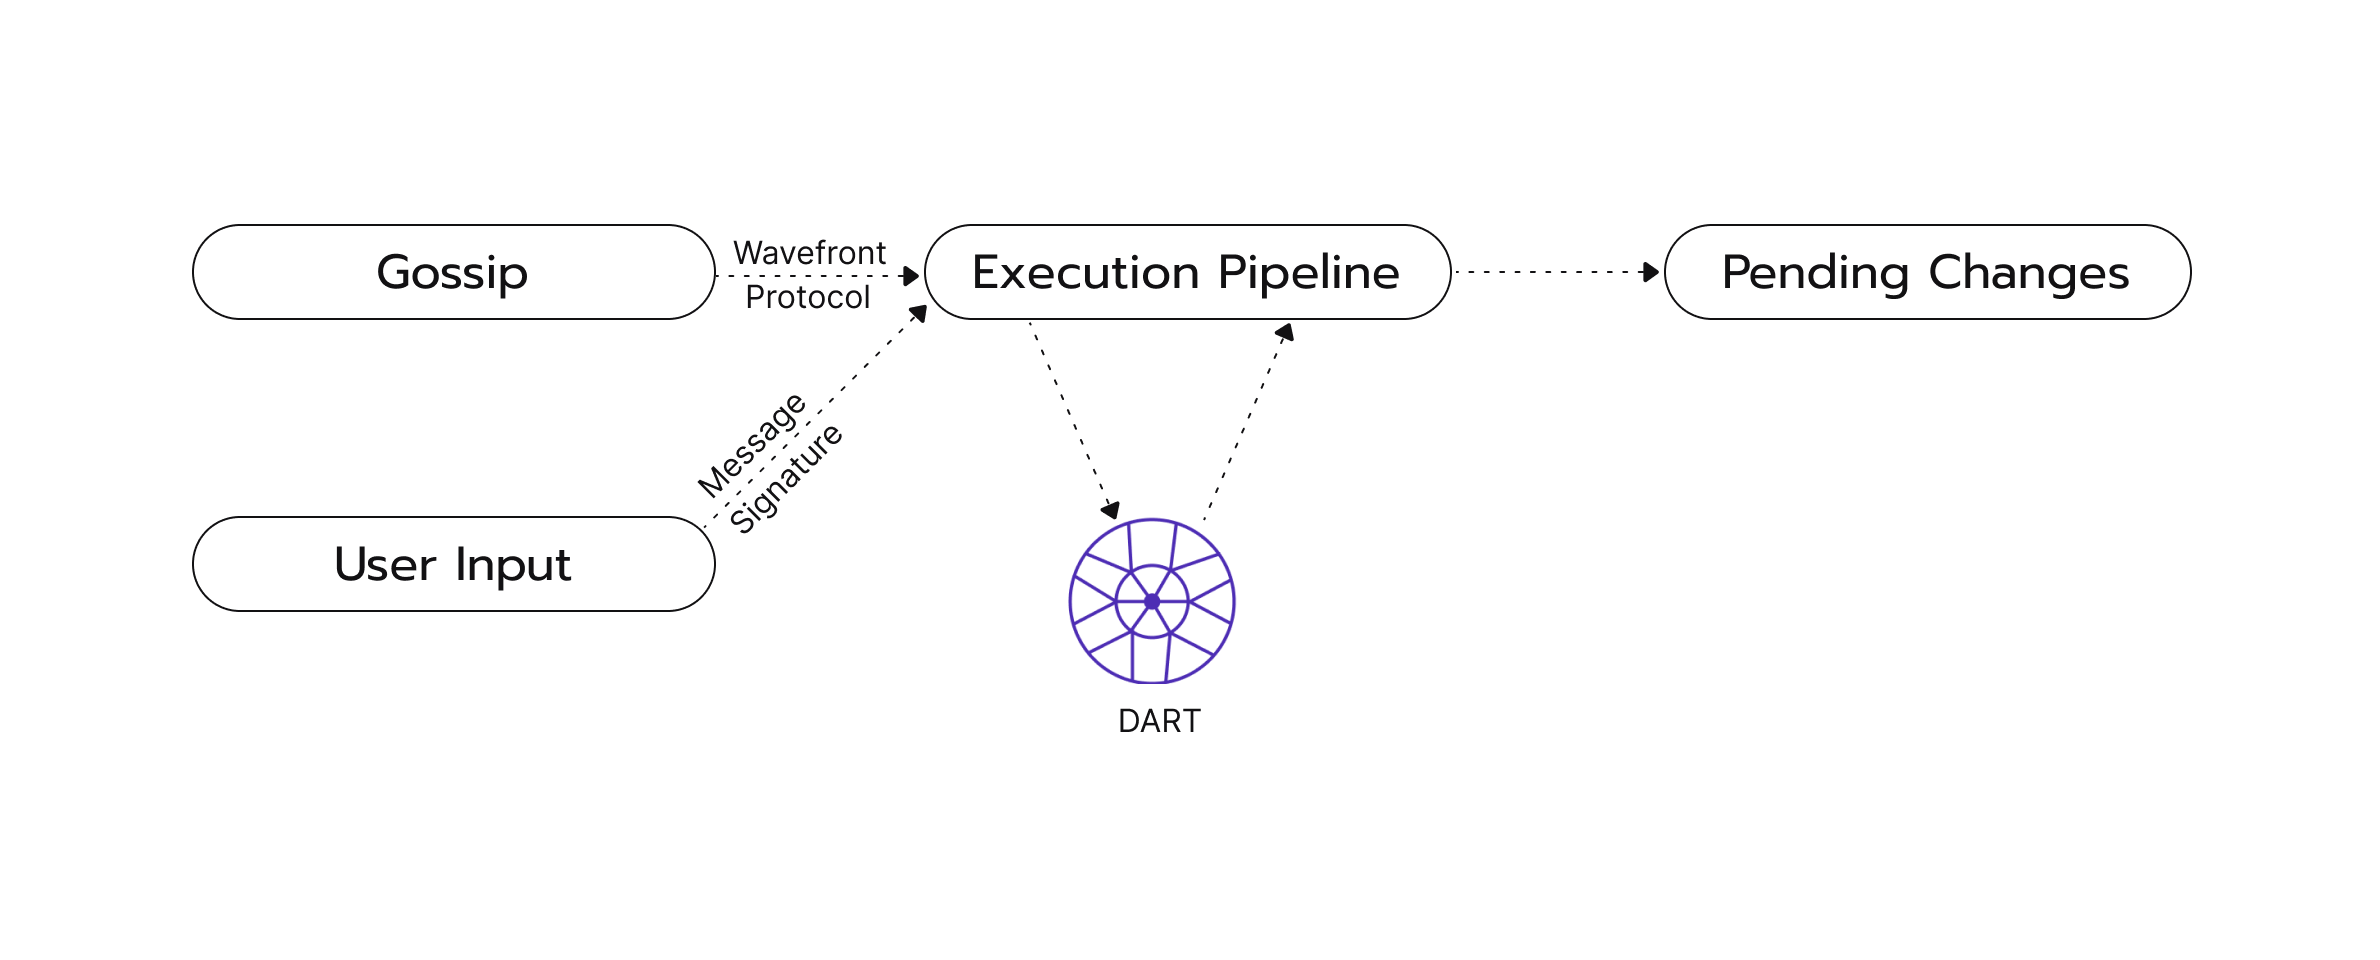
\includegraphics[width=1.2\textwidth,center]{figures/signature_zoom.png}
        \caption{A technical close-up of how nodes handle receiving information.}
        \label{figure:signature_zoom}
    \end{figure}

\pagebreak

\subsection{Node POV: Epoch and Consensus}
    Epochs occur continuously as the consensus protocol runs, and is when events are finally and irreversibly agreed upon. Once an epoch occurs in the consensus protocol (the Hashgraph) this epoch is passed into an ordered execution. This module orders all the events contained in this epoch, and checks for double spending. It then passes all valid outputs to the \gls{dart}. The \gls{dart} deletes all inputs of the executed smart contracts, and writes all outputs of the smart contracts. At this point, all valid smart contracts have been executed on the \gls{dart}. Once this has been done, a \gls{bullseye} representing the state of the system is computed. This \gls{bullseye} is then signed and gossiped to the rest of the nodes. This allows nodes to check their local \gls{dart} against others, making sure the system is running smoothly, or figuring out if it has made a local error itself.
    \begin{figure}[H]
        \centering
        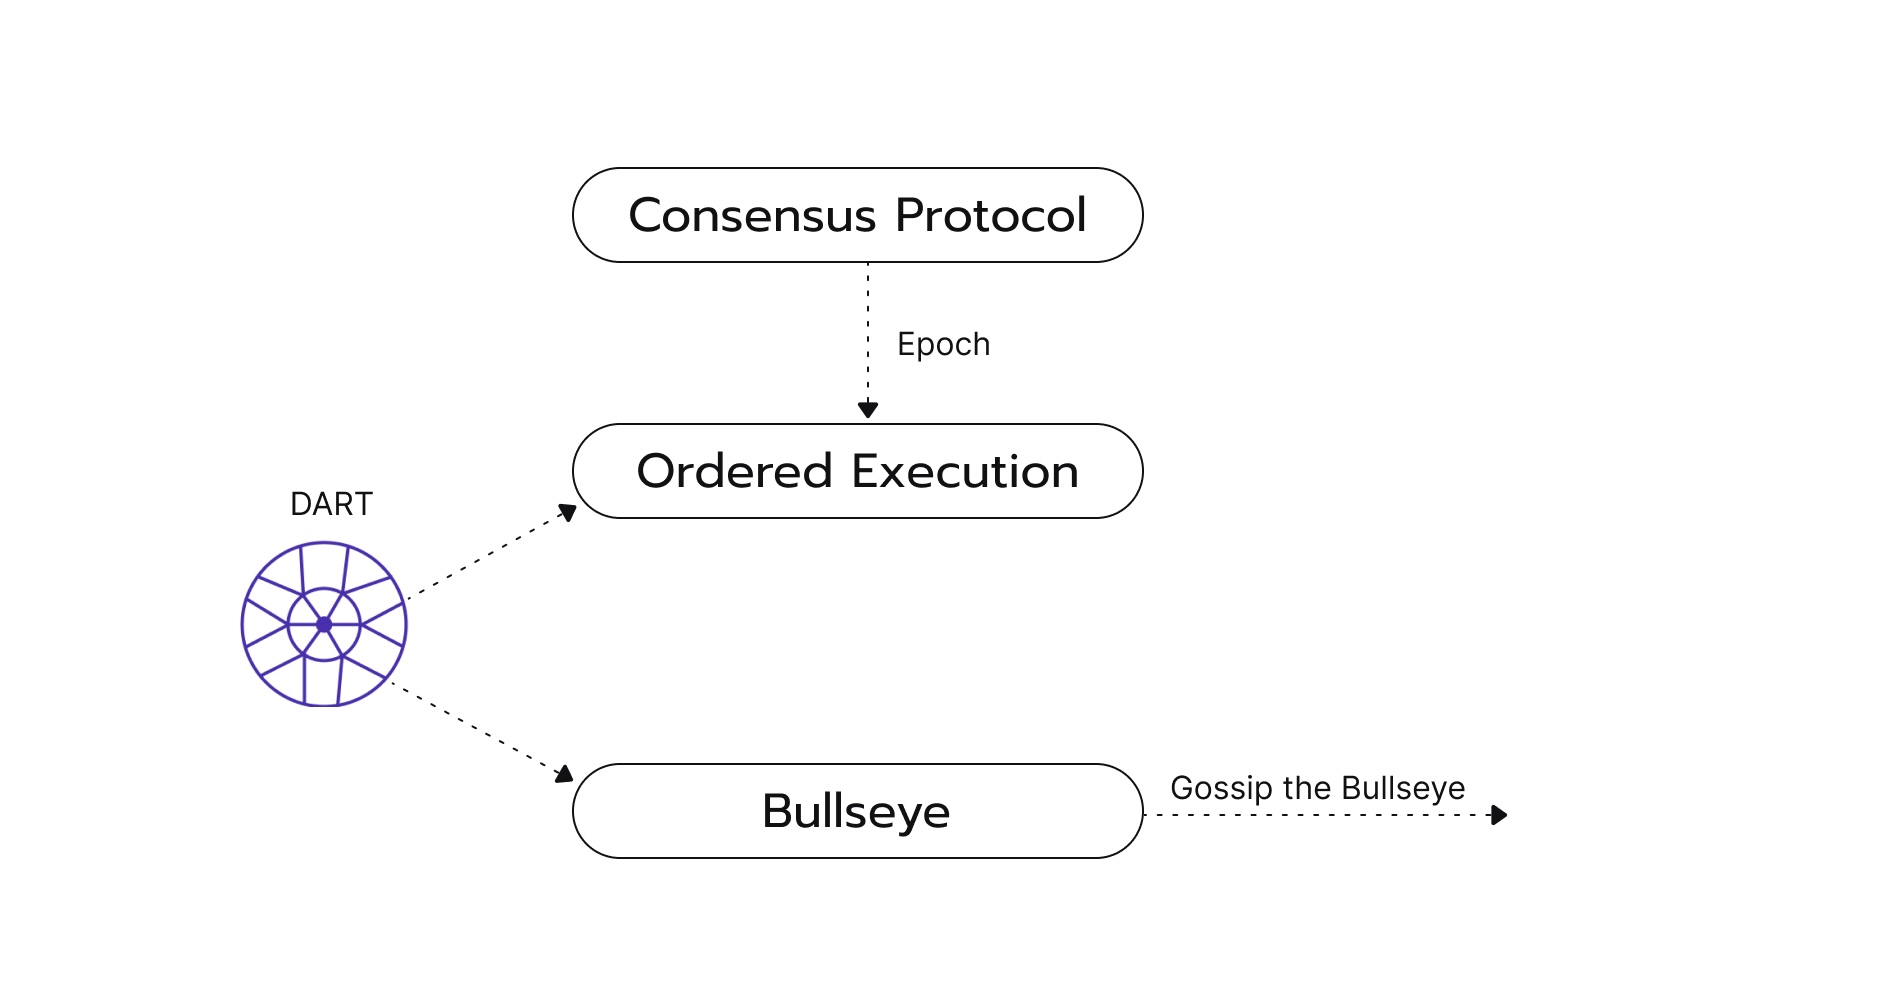
\includegraphics[width=1.2\textwidth,center]{figures/epoch_zoom.jpeg}
        \caption{A close-up of what happens when an epoch occurs.}
        \label{figure:epoch_zoom}
    \end{figure}

\subsection{Comparison to Blockchain Systems}
    Blockchain systems fundamentally tie the consensus layer to the storage layer. The longest chain of stored data is what defines the consensus. Tagion is fundamentally different. In the Tagion system, the consensus algorithm and the storage layer are distinct parts. The consensus occurs in the Hashgraph, and the data is stored in the \gls{dart}. This structure allows us to make the consensus layer, and the storage layer, separately much faster than they could be when jumbled together. This is what really allows Tagion to achieve scalability, without compromising on any parts of the \gls{trilemma}.

\pagebreak